\chapter{Toán tử, đại lượng quan sát và các ma trận Pauli}

Ký hiệu tốt không phải là thứ trang trí. Trong một môn học được xây dựng từ các vectơ trừu tượng và các số phức, một hệ ký hiệu cho phép ta thao tác với các ký hiệu mà không phải liên tục diễn chúng thành lời là một phần của chính bộ công cụ. Ký hiệu bra--ket của Dirac có giá trị chính vì lý do đó: nó làm cho hình học của không gian trạng thái vẫn hiển lộ đồng thời cho phép ta tính toán bằng các thành phần và ma trận.

Nhiệm vụ trước mắt của chúng ta là về mặt toán học. Ta sẽ giới thiệu các toán tử tuyến tính, tìm hiểu cách chúng tác dụng lên bra cũng như ket, và tách riêng lớp đặc biệt gọi là các toán tử Hermite. Chỉ khi đó ta mới gắn cho chúng các từ ngữ vật lý \emph{đại lượng quan sát}, \emph{kết quả đo}, và \emph{xác suất}. Phần thưởng là ba đại lượng quan sát spin xuất hiện như các ma trận Pauli thay vì được trao cho ta như những đối tượng phải ghi nhớ.

\section{Cơ sở trực chuẩn và các thành phần}

Các trạng thái tạo thành một không gian vectơ tuyến tính phức. Các vectơ ket của nó có thể được cộng với nhau và nhân với các số phức. Gắn với mỗi ket \(\ket{A}\) là một bra \(\bra{A}\), thu được bằng phép liên hợp đối ngẫu. Một cơ sở không là duy nhất, nhưng một khi đã chọn thì mọi vectơ đều có thể được mô tả bằng các thành phần của nó trong cơ sở đó.

Cho
\[
\bigl\{\ket{1},\ket{2},\ldots,\ket{N}\bigr\}
\]
là một cơ sở trực chuẩn. Tính trực giao và chuẩn hóa được tóm tắt bởi
\begin{equation}
\braket{j}{i}=\delta_{ji}.
\label{eq:orthonormal-basis}
\end{equation}
Ở đây \(\delta_{ji}\) bằng một khi \(j=i\) và bằng không trong các trường hợp khác. Số chiều \(N\) là số lớn nhất các hướng đôi một trực giao trong không gian; một cơ sở trực chuẩn đầy đủ chứa đúng bấy nhiêu vectơ.

Khai triển một ket bất kỳ dưới dạng
\begin{equation}
\ket{A}=\sum_i \alpha_i\ket{i}.
\label{eq:ket-expansion}
\end{equation}
Các hệ số không có gì bí ẩn. Nhân từ bên trái với \(\bra{j}\):
\begin{align}
\braket{j}{A}
 &=\sum_i\alpha_i\braket{j}{i} \\
 &=\sum_i\alpha_i\delta_{ji}
 =\alpha_j.
\end{align}
Do đó
\begin{equation}
\alpha_i=\braket{i}{A}.
\label{eq:components-inner-products}
\end{equation}
Thành phần thứ \(i\) là hình chiếu của \(\ket{A}\) lên hướng cơ sở thứ \(i\).

Thế Phương trình~\eqref{eq:components-inner-products} trở lại vào Phương trình~\eqref{eq:ket-expansion} cho dạng đặc biệt hữu ích
\begin{equation}
\ket{A}=\sum_i\ket{i}\braket{i}{A}.
\label{eq:ket-completeness-action}
\end{equation}
Tổng này không làm gì với vectơ; nó chỉ phân giải vectơ theo các hướng cơ sở của nó rồi ghép lại. Ta sẽ dùng phép toán này lặp đi lặp lại. Nó thường được mô tả là \emph{chèn một hệ đầy đủ các trạng thái}, bởi vì
\begin{equation}
\sum_i\ket{i}\bra{i}=\mathbf 1.
\label{eq:resolution-identity}
\end{equation}

Khai triển bra tương ứng là
\begin{equation}
\bra{A}=\sum_i\braket{A}{i}\bra{i}
       =\sum_i\alpha_i^*\bra{i}.
\label{eq:bra-expansion}
\end{equation}
Liên hợp phức trên \(\alpha_i\) là thiết yếu. Việc biến một ket thành một bra sẽ liên hợp mọi hệ số bằng số.

\begin{figure}[htbp]
\centering
\includegraphics[width=0.82\textwidth]{lecture_03_figure_04.png}
\caption{Hai quy tắc định nghĩa của một toán tử tuyến tính, được viết ra sau phần ôn lại về cơ sở.}
\lectureframe{00:12:44}
\end{figure}

\section{Toán tử tuyến tính như những cỗ máy}

Một toán tử tuyến tính \(M\) là một quy tắc đưa một ket đầu vào thành một ket đầu ra duy nhất. Một hình dung hữu ích, do John Wheeler đề xuất, là một cỗ máy có cổng vào và cổng ra: đưa \(\ket{A}\) vào, quay bánh xe, và nhận \(M\ket{A}\). Đầu ra được xác định bởi đầu vào. Chiều ngược lại không nhất thiết là duy nhất; hai đầu vào có thể cho cùng một đầu ra, và một cỗ máy nghịch đảo có thể không tồn tại.

Tính từ \emph{tuyến tính} gồm hai quy tắc. Với một số phức \(z\),
\begin{align}
M\bigl(z\ket{A}\bigr)&=z\,M\ket{A}, \label{eq:operator-homogeneous}\\
M\bigl(\ket{A}+\ket{B}\bigr)&=M\ket{A}+M\ket{B}.
\label{eq:operator-additive}
\end{align}
Một vô hướng đi qua cỗ máy mà không đổi, và một tổng có thể được xử lý từng hạng một. Những quy tắc này cũng suy ra tính tuyến tính đối với mọi tổ hợp tuyến tính phức hữu hạn.

Ý tưởng ấy cũng áp dụng cho các vectơ ba chiều thông thường. Cơ học lượng tử không phát minh ra các ánh xạ tuyến tính. Nó làm cho chúng trở nên không thể thiếu vì không gian trạng thái là trừu tượng và phức, và vì các đại lượng đo được sẽ được biểu diễn bởi một họ đặc biệt của những ánh xạ như vậy.

\section{Từ một toán tử đến ma trận của nó}

Giả sử cỗ máy đưa \(\ket{A}\) thành \(\ket{B}\):
\begin{equation}
M\ket{A}=\ket{B}.
\label{eq:operator-action}
\end{equation}
Hãy chọn cùng một cơ sở trực chuẩn cho đầu vào và đầu ra, rồi viết
\[
\ket{A}=\sum_j\alpha_j\ket{j},
\qquad
\ket{B}=\sum_i\beta_i\ket{i}.
\]
Để tìm thành phần đầu ra thứ \(i\), chiếu Phương trình~\eqref{eq:operator-action} bằng \(\bra{i}\):
\begin{equation}
\bra{i}M\ket{A}=\braket{i}{B}=\beta_i.
\end{equation}
Bây giờ chèn khai triển của \(\ket{A}\):
\begin{align}
\bra{i}M\ket{A}
 &=\sum_j\bra{i}M\ket{j}\braket{j}{A}\\
 &=\sum_j\bra{i}M\ket{j}\alpha_j
 =\beta_i.
\end{align}
Các số
\begin{equation}
m_{ij}\equiv\bra{i}M\ket{j}
\label{eq:matrix-elements}
\end{equation}
là \emph{phần tử ma trận} của \(M\) trong cơ sở đã chọn. Do đó,
\begin{equation}
\boxed{\sum_jm_{ij}\alpha_j=\beta_i.}
\label{eq:component-action}
\end{equation}

\begin{figure}[htbp]
\centering
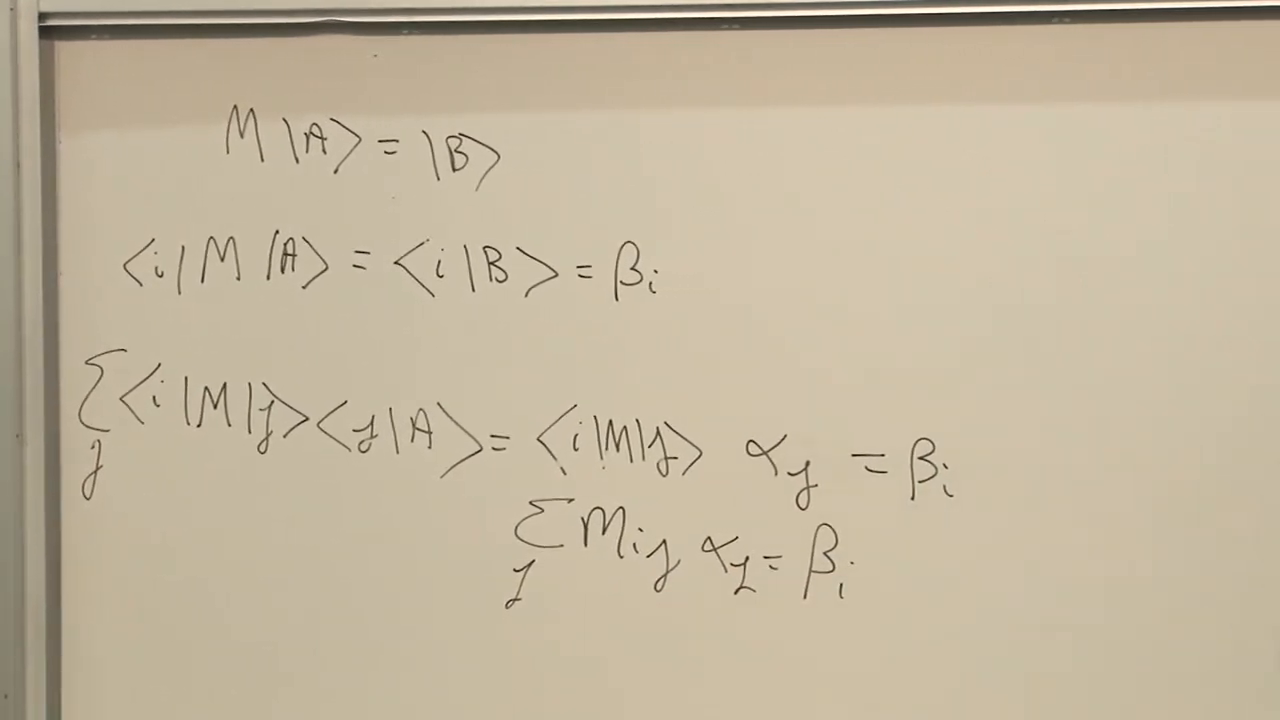
\includegraphics[width=0.84\textwidth]{lecture_03_figure_02.png}
\caption{Phương trình trừu tượng \(M\ket{A}=\ket{B}\) được chiếu và phân giải thành quy tắc thành phần \(\sum_jm_{ij}\alpha_j=\beta_i\).}
\lectureframe{00:18:30}
\end{figure}

Nếu không gian có số chiều \(N\), thì \(N^2\) số \(m_{ij}\) tạo thành một ma trận vuông \(N\times N\). Phương trình~\eqref{eq:component-action} chính là
\begin{equation}
\begin{pmatrix}
m_{11}&m_{12}&\cdots&m_{1N}\\
m_{21}&m_{22}&\cdots&m_{2N}\\
\vdots&\vdots&\ddots&\vdots\\
m_{N1}&m_{N2}&\cdots&m_{NN}
\end{pmatrix}
\begin{pmatrix}
\alpha_1\\
\alpha_2\\
\vdots\\
\alpha_N
\end{pmatrix}
=
\begin{pmatrix}
\beta_1\\
\beta_2\\
\vdots\\
\beta_N
\end{pmatrix}.
\label{eq:matrix-vector-action}
\end{equation}
Để thu được \(\beta_1\), hãy nhân hàng thứ nhất với cột đầu vào rồi cộng lại; lặp lại với hàng thứ hai để được \(\beta_2\), và cứ thế tiếp tục. Ma trận là phiên bản cụ thể của cỗ máy Wheeler.

\begin{figure}[htbp]
\centering
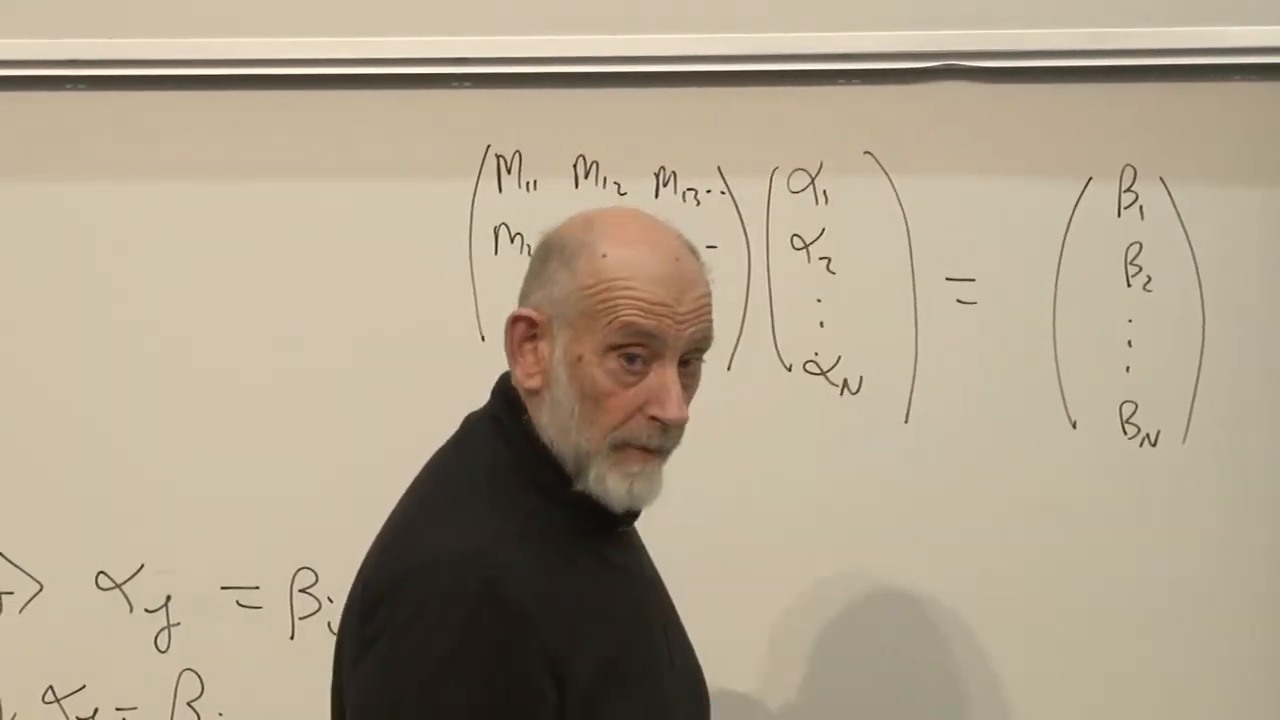
\includegraphics[width=0.84\textwidth]{lecture_03_figure_03.png}
\caption{Cùng một tác dụng của toán tử được biểu diễn dưới dạng một ma trận vuông nhân với cột hệ số đầu vào.}
\lectureframe{00:20:01}
\end{figure}

Ta đã thu được một thuật toán và đánh mất phần nào hình học trực quan. Mệnh đề trừu tượng \(M\ket{A}=\ket{B}\) không phụ thuộc vào tọa độ. Các phần tử cụ thể \(m_{ij}\), \(\alpha_j\) và \(\beta_i\) thì có phụ thuộc vào cơ sở đã chọn. Một cơ sở trực chuẩn khác sẽ làm thay đổi cả ba dãy này trong khi vẫn giữ nguyên ánh xạ nền tảng và các dự đoán vật lý của nó.

\begin{classroomqa}
\audiencequestion{Việc chọn cơ sở có thể quyết định một bài toán có giải được hay không?}
\lecturerresponse{Nó có thể quyết định liệu lời giải có dễ nhìn ra hay không. Một cơ sở được chọn khéo có thể làm cho một toán tử trở thành đường chéo và khiến phép tính gần như tức thì; một cơ sở tồi có thể che khuất cấu trúc dưới lớp đại số khó chịu. Nó không thể làm thay đổi kết quả của một thí nghiệm. Nếu hai cơ sở dẫn đến hai câu trả lời vật lý khác nhau, thì phép tính đã sai.}
\end{classroomqa}

\section{Bra, ket và tính phản tuyến tính}

\begin{classroomqa}
\audiencequestion{Một toán tử tuyến tính có thể biến một ket thành một bra, hoặc một bra thành một ket không?}
\lecturerresponse{Không phải một toán tử tuyến tính thông thường thuộc loại vừa định nghĩa. Nó ánh xạ ket thành ket, với các vô hướng phức đi qua mà không đổi. Phép toán hoán đổi ket và bra cũng đồng thời liên hợp phức các hệ số của chúng, nên nó thuộc về một lớp khác.}
\end{classroomqa}

Phép nhân với một số phức cố định là một toán tử tuyến tính đơn giản. Phép liên hợp phức thì không. Nếu \(K\) ký hiệu phép liên hợp, thì
\[
K\bigl(z\ket{A}\bigr)=z^*K\ket{A},
\]
chứ không phải \(zK\ket{A}\). Một ánh xạ như vậy được gọi là \emph{phản tuyến tính}. Tên gọi này không có nghĩa là đối lập với tuyến tính; nó ghi nhận việc liên hợp các vô hướng. Mối liên hệ sâu hơn của nó với phản hạt vượt ra ngoài cuộc thảo luận hiện tại.

Tuy vậy, vẫn có thể để các toán tử tuyến tính tác dụng lên bra. Theo quy ước, toán tử được viết ở bên phải:
\begin{equation}
\bra{A}M.
\end{equation}
Định nghĩa này được chọn sao cho một phần tử ma trận không còn mơ hồ về dấu ngoặc:
\begin{equation}
\bra{A}\bigl(M\ket{B}\bigr)
=
\bigl(\bra{A}M\bigr)\ket{B}
\equiv
\bra{A}M\ket{B}.
\label{eq:bracket-independence}
\end{equation}

Để thấy vì sao điều này là khả dĩ, hãy khai triển cả hai vectơ:
\begin{align}
\bra{A}M\ket{B}
 &=\left(\sum_i\alpha_i^*\bra{i}\right)
   M
   \left(\sum_j\beta_j\ket{j}\right)\\
 &=\sum_{ij}\alpha_i^*m_{ij}\beta_j.
\label{eq:matrix-element-double-sum}
\end{align}
Đây là một tổng kép thông thường. Ta có thể cộng theo \(j\) trước và xem \(M\) tác dụng lên ket, hoặc cộng theo \(i\) trước và xem nó tác dụng lên bra. Kết quả là như nhau. Ký hiệu được sắp đặt theo cách này chính là để có thể bỏ đi những dấu ngoặc không cần thiết.

\section{Phép toán dagger}

Có một câu hỏi thứ hai, khác đi, ở phía bra. Giả sử
\[
M\ket{A}=\ket{B}.
\]
Toán tử nào biến bra tương ứng \(\bra{A}\) thành \(\bra{B}\)? Nói chung, đó không phải chính \(M\). Nếu \(M\) là phép nhân với một số phức \(z\), thì phương trình ket sẽ là \(\ket{B}=z\ket{A}\), còn phương trình bra sẽ là \(\bra{B}=z^*\bra{A}\).

Toán tử cần tìm được ký hiệu là \(M^\dagger\), \emph{liên hợp Hermite} của \(M\), và được định nghĩa bởi
\begin{equation}
M\ket{A}=\ket{B}
\quad\Longleftrightarrow\quad
\bra{A}M^\dagger=\bra{B}.
\label{eq:dagger-definition}
\end{equation}
Phép dagger là phép tương tự ở mức toán tử của phép liên hợp phức.

Quy tắc ma trận của nó suy ra trực tiếp. Cho
\[
M\ket{i}=\ket{i'}.
\]
Khi đó
\[
m_{ji}=\bra{j}M\ket{i}=\braket{j}{i'}.
\]
Quan hệ bra sau khi lấy dagger là \(\bra{i}M^\dagger=\bra{i'}\), nên
\[
(m^\dagger)_{ij}
=\bra{i}M^\dagger\ket{j}
=\braket{i'}{j}.
\]
Đảo thứ tự một tích vô hướng sẽ liên hợp phức nó:
\[
\braket{i'}{j}=\braket{j}{i'}^*.
\]
Vì thế
\begin{equation}
\boxed{(m^\dagger)_{ij}=m_{ji}^*.}
\label{eq:dagger-matrix-elements}
\end{equation}

\begin{figure}[htbp]
\centering
\includegraphics[width=0.84\textwidth]{lecture_03_figure_05.png}
\caption{Quan hệ hoàn chỉnh trên bảng cho liên hợp Hermite: đổi chỗ các chỉ số và lấy liên hợp phức.}
\lectureframe{00:42:23}
\end{figure}

Trong ngôn ngữ ma trận, ta chuyển vị rồi lấy liên hợp phức:
\begin{equation}
\begin{pmatrix}
a&b\\
c&d
\end{pmatrix}^{\!\dagger}
=
\begin{pmatrix}
a^*&c^*\\
b^*&d^*
\end{pmatrix}.
\label{eq:dagger-two-by-two}
\end{equation}
Phép chuyển vị phản chiếu các phần tử qua đường chéo chính; phép liên hợp thay mỗi \(i\) bằng \(-i\). Ví dụ,
\begin{equation}
\begin{pmatrix}
2&6+7i\\
4-i&9+i
\end{pmatrix}^{\!\dagger}
=
\begin{pmatrix}
2&4+i\\
6-7i&9-i
\end{pmatrix}.
\label{eq:dagger-numerical-example}
\end{equation}
Các phần tử trên đường chéo vẫn giữ nguyên vị trí nhưng được liên hợp, còn hai phần tử ngoài đường chéo thì đổi chỗ cho nhau và được liên hợp.

\section{Toán tử Hermite}

Một số phức là số thực đúng khi và chỉ khi nó bằng chính liên hợp phức của nó. Sự tương tự ở mức toán tử là hiển nhiên.

\begin{definition}
Một toán tử \(M\) là \emph{Hermite} khi
\begin{equation}
M=M^\dagger.
\label{eq:hermitian-definition}
\end{equation}
Tương đương, trong mọi cơ sở trực chuẩn,
\begin{equation}
m_{ij}=m_{ji}^*.
\label{eq:hermitian-components}
\end{equation}
\end{definition}

Đặt \(i=j\) trong Phương trình~\eqref{eq:hermitian-components}. Khi đó
\[
m_{ii}=m_{ii}^*,
\]
nên mọi phần tử trên đường chéo đều là số thực. Ngoài đường chéo, các phần tử xuất hiện thành những cặp phản chiếu liên hợp. Nếu một phần tử là \(4-i\) thì phần tử phản chiếu tương ứng của nó là \(4+i\); nếu một phần tử là số thực \(5\) thì phần tử tương ứng của nó cũng vậy.

\begin{figure}[htbp]
\centering
\includegraphics[width=0.78\textwidth]{lecture_03_figure_06.png}
\caption{Một ví dụ ma trận Hermite hoàn chỉnh: các phần tử thực trên đường chéo và các cặp liên hợp phức phản chiếu qua nó.}
\lectureframe{00:45:43}
\end{figure}

Các toán tử Hermite quan trọng vì chúng sẽ biểu diễn các đại lượng đo được. Trước khi thực hiện sự đồng nhất đó, ta cần hiểu các hướng riêng của chúng.

\section{Vectơ riêng và hướng riêng}

Lần đầu gặp vectơ riêng có thể khiến phần này có vẻ đi nhanh hơn phần vật lý xung quanh nó. Các ý tưởng ở đây thuộc đại số tuyến tính chuẩn tắc chứ không phải một giả thuyết vật lý mới; nếu chúng còn lạ lẫm, thì nên bình tĩnh ôn lại các định nghĩa rồi quay lại lập luận.

Một toán tử tổng quát làm thay đổi hướng của một vectơ. Chẳng hạn, một phép quay trong không gian ba chiều thông thường làm cho hầu như mọi vectơ lệch khỏi chính hướng ban đầu của nó. Trục quay là ngoại lệ: một vectơ nằm dọc theo trục đó trở lại theo cùng hướng. Đó là mô hình cho một vectơ riêng.

Một phép quay không tầm thường của một mặt phẳng thực hai chiều minh họa khả năng ngược lại: không có hướng thực nào còn được giữ nguyên đến một hệ số tỉ lệ thực. Vì vậy, một toán tử tổng quát trên một không gian thực bị giới hạn không nhất thiết phải có vectơ riêng thực. Các toán tử Hermite trên những không gian trạng thái phức được dùng trong cơ học lượng tử có những tính chất mạnh hơn nhiều.

Một vectơ riêng của \(M\) thỏa mãn
\begin{equation}
M\ket{i}=\lambda_i\ket{i}.
\label{eq:eigenvalue-equation}
\end{equation}
Số \(\lambda_i\) là trị riêng của nó. Vectơ riêng gắn với toán tử; người ta không nói đến một vectơ riêng mà không chỉ rõ ánh xạ mà nó bảo toàn hướng.

Độ dài và pha của nó không được cố định bởi Phương trình~\eqref{eq:eigenvalue-equation}. Với mọi số phức khác không \(z\),
\[
M\bigl(z\ket{i}\bigr)
=zM\ket{i}
=\lambda_i\bigl(z\ket{i}\bigr).
\]
Vì vậy, nói đến một \emph{hướng riêng} sẽ chính xác hơn: mọi bội khác không của \(\ket{i}\) đều mô tả cùng một hướng và mang cùng một trị riêng. Ta thường chọn một đại diện đã chuẩn hóa.

Sự kiện phổ trung tâm là như sau: một toán tử Hermite trên một không gian vectơ phức có số chiều \(N\) có một cơ sở trực chuẩn đầy đủ gồm \(N\) vectơ riêng. Hai phần của mệnh đề đó có thể thấy được chỉ với rất ít đại số.

\subsection{Các trị riêng của toán tử Hermite là số thực}

Giả sử \(M=M^\dagger\) và
\[
M\ket{i}=\lambda_i\ket{i}.
\]
Lấy liên hợp Hermite của toàn bộ phương trình:
\begin{equation}
\bra{i}M^\dagger=\lambda_i^*\bra{i}.
\label{eq:eigen-bra-equation}
\end{equation}
Vì \(M^\dagger=M\), hãy nhân phương trình ket với \(\bra{i}\) và phương trình bra với \(\ket{i}\):
\begin{align}
\bra{i}M\ket{i}&=\lambda_i\braket{i}{i},\\
\bra{i}M\ket{i}&=\lambda_i^*\braket{i}{i}.
\end{align}
Cùng một chuẩn khác không nhân với cả hai số, nên
\begin{equation}
\lambda_i=\lambda_i^*.
\end{equation}
Mọi trị riêng của một toán tử Hermite đều là số thực. Đây là gợi ý đầu tiên cho thấy một toán tử như vậy có thể biểu diễn con số thực hiển thị trên một thiết bị đo.

\subsection{Các trị riêng khác nhau cho các vectơ riêng trực giao}

Cho
\[
M\ket{i}=\lambda_i\ket{i},
\qquad
M\ket{j}=\lambda_j\ket{j},
\]
trong đó \(M\) là Hermite. Lấy liên hợp Hermite của phương trình thứ hai. Ta đã biết trị riêng của nó là số thực:
\[
\bra{j}M=\lambda_j\bra{j}.
\]
Bây giờ nhân phương trình thứ nhất với \(\bra{j}\) và phương trình bra với \(\ket{i}\):
\begin{align}
\bra{j}M\ket{i}&=\lambda_i\braket{j}{i},\\
\bra{j}M\ket{i}&=\lambda_j\braket{j}{i}.
\end{align}
Lấy hiệu, ta được
\begin{equation}
\boxed{(\lambda_i-\lambda_j)\braket{j}{i}=0.}
\label{eq:hermitian-orthogonality}
\end{equation}
Nếu \(\lambda_i\ne\lambda_j\), thì
\[
\braket{j}{i}=0.
\]
Các hướng riêng trực giao với nhau.

\begin{figure}[htbp]
\centering
\includegraphics[width=0.82\textwidth]{lecture_03_figure_07.png}
\caption{Dòng then chốt trong chứng minh tính trực giao: các trị riêng không bằng nhau buộc tích vô hướng phải triệt tiêu.}
\lectureframe{00:59:00}
\end{figure}

Khi hai trị riêng tình cờ bằng nhau, Phương trình~\eqref{eq:hermitian-orthogonality} không áp đặt điều kiện nào bên trong không gian riêng suy biến đó. Ta có thể chọn ở đó một cơ sở trực chuẩn. Cùng với các phương riêng còn lại, các vectơ ấy tạo thành cơ sở trực chuẩn đầy đủ gồm các vectơ riêng mà định lý phổ bảo đảm.

Tính trực giao cũng có một cách diễn giải vật lý. Hai trạng thái trực giao có thể được phân biệt không mơ hồ bằng một phép đo thích hợp. Các trạng thái riêng ứng với các trị riêng khác nhau phải phân biệt được vì thiết bị cho ra các số thực khác nhau đối với chúng. Đại số và ý nghĩa thao tác đã cùng chỉ đến cùng một sự tương ứng.

\section{Các tiên đề về phép đo}

Chúng ta giờ đã có đủ hình thức toán học để phát biểu các sự tương ứng cơ bản của cơ học lượng tử. Lần đầu gặp chúng, ta có thể thấy chúng xa lạ. Ý nghĩa của chúng chỉ trở nên cụ thể sau khi được sử dụng, vì vậy hãy phát biểu chúng thật gọn gàng rồi lập tức quay lại thí nghiệm spin.

Một phép đo đơn lẻ cho ra một số thực. Ta có thể gộp hai kết quả đọc số thực tương thích thành một số phức, nhưng gói đó vẫn chứa hai phép đo. Đầu ra cơ bản của một bộ dò là số thực. Vì thế, các toán tử Hermite là những ứng viên tự nhiên: các trị riêng của chúng là số thực, và các vectơ riêng của chúng tạo thành một cơ sở trực chuẩn đầy đủ.

\begin{enumerate}
\item Một đại lượng đo được, hay \emph{đại lượng quan sát}, được biểu diễn bởi một toán tử Hermite \(M\).
\item Các kết quả có thể có khi đo \(M\) là các trị riêng \(\lambda_i\) của nó.
\item Một trạng thái mà trong đó \(M\) có giá trị xác định \(\lambda_i\) là một trạng thái riêng \(\ket{i}\) thỏa mãn
\[
M\ket{i}=\lambda_i\ket{i}.
\]
\item Nếu hệ ở trong một trạng thái chuẩn hóa tổng quát \(\ket{A}\), thì xác suất thu được \(\lambda_i\) là
\begin{equation}
P(\lambda_i\mid A)
=\left|\braket{i}{A}\right|^2
=\braket{i}{A}\braket{A}{i}.
\label{eq:born-rule}
\end{equation}
\end{enumerate}

Danh sách này là một điểm khởi đầu thuận tiện, không nhất thiết là một hệ tiên đề độc lập tối thiểu; với một cách phát biểu tiết kiệm hơn, một số mệnh đề có thể được suy ra từ những mệnh đề khác. Giữ riêng các sự tương ứng làm cho vai trò vật lý của chúng dễ thấy hơn.

Số phức \(\braket{i}{A}\) là một \emph{biên độ xác suất}, không phải xác suất. Nhân nó với liên hợp phức của nó cho ra một số thực không âm. Đối với một thành phần spin, phổ chỉ có hai giá trị, \(+1\) và \(-1\); một đại lượng quan sát tổng quát hơn có thể có nhiều trị riêng.

\begin{figure}[htbp]
\centering
\includegraphics[width=0.82\textwidth]{lecture_03_figure_08.png}
\caption{Nội dung trên bảng liên hệ các trạng thái cho kết quả xác định với các vectơ riêng, và liên hệ xác suất của \(\lambda_i\) với bình phương độ lớn của hình chiếu lên \(\ket{i}\).}
\lectureframe{01:11:29}
\end{figure}

\begin{classroomqa}
\audiencequestion{Chính xác thì bên cạnh \(P\) trong quy tắc xác suất viết gì?}
\lecturerresponse{Đó là \(\lambda_i\): \(P(\lambda_i\mid A)\) có nghĩa là xác suất để một phép đo của \(M\), khi hệ được chuẩn bị trong \(\ket{A}\), trả về đúng trị riêng \(\lambda_i\). Vế phải là bình phương độ lớn của hình chiếu lên vectơ riêng đó.}
\end{classroomqa}

\subsection{Chuẩn hóa và tính đầy đủ}

Các xác suất của mọi kết quả loại trừ lẫn nhau phải cộng lại thành một:
\begin{equation}
\sum_i\left|\braket{i}{A}\right|^2=1.
\label{eq:probability-normalization}
\end{equation}
Chèn cơ sở riêng đầy đủ vào:
\begin{align}
\sum_i\left|\braket{i}{A}\right|^2
 &=\sum_i\braket{A}{i}\braket{i}{A}\\
 &=\bra{A}\left(\sum_i\ket{i}\bra{i}\right)\ket{A}\\
 &=\braket{A}{A}.
\end{align}
Do đó một vectơ trạng thái hợp lệ phải được chuẩn hóa,
\begin{equation}
\braket{A}{A}=1.
\label{eq:state-normalization}
\end{equation}
Nếu \(\ket{A}=\sum_i\alpha_i\ket{i}\), thì cùng điều kiện ấy là
\begin{equation}
\sum_i\alpha_i^*\alpha_i=1.
\label{eq:component-normalization}
\end{equation}
Đây là một ràng buộc thực lên các thành phần phức.

\begin{classroomqa}
\audiencequestion{Mọi xác suất có bắt buộc phải dương không?}
\lecturerresponse{Có. Mỗi xác suất là một số nhân với liên hợp phức của chính nó, nên nó không âm. Khi đó điều kiện chuẩn hóa làm cho tổng của mọi số như vậy bằng một.}
\end{classroomqa}

Còn có một tính dư thừa khác. Nhân mọi thành phần với cùng một pha,
\begin{equation}
\ket{A}\longmapsto e^{i\theta}\ket{A},
\label{eq:l3-global-phase}
\end{equation}
sẽ nhân mọi biên độ với \(e^{i\theta}\) và để nguyên mọi bình phương độ lớn. Không phép đo nào có thể phát hiện pha chung đó. Các pha tương đối giữa các thành phần vẫn mang ý nghĩa vật lý; chỉ một pha nhân lên toàn bộ trạng thái mới là dư thừa.

Vì vậy, hai tham số thực trong một vectơ phức tùy ý không xác định trạng thái vật lý: độ lớn của nó bị cố định bởi điều kiện chuẩn hóa, còn pha toàn cục của nó thì không quan sát được. Đây chính là số lượng tham số đã gặp đối với một spin đơn lẻ, nay được suy ra từ quy tắc xác suất tổng quát.

\subsection{Phép đo cũng chuẩn bị trạng thái}

Có thêm một tiên đề nữa, nói ra thì dễ hơn là nén vào một dòng ngắn trên bảng. Nếu một phép đo cho ra \(\lambda_i\), thì ngay sau đó hệ ở trong trạng thái riêng tương ứng \(\ket{i}\). Thiết bị vừa ghi nhận một kết quả, vừa chuẩn bị một trạng thái mà trong đó việc lặp lại cùng phép đo sẽ cho kết quả xác định ấy.

\begin{classroomqa}
\audiencequestion{Có thể nhắc lại thêm một lần mệnh đề phép đo-chuẩn bị đó không?}
\lecturerresponse{Trước phép đo, một số trị riêng có thể xuất hiện với các xác suất trong Phương trình~\eqref{eq:born-rule}. Một khi thiết bị thực sự báo \(\lambda_i\), hệ được để lại trong trạng thái riêng ứng với \(\lambda_i\). Vì thế, một phép đo thứ hai ngay lập tức của cùng đại lượng quan sát sẽ trả về cùng giá trị.}
\end{classroomqa}

\begin{classroomqa}
\audiencequestion{Các nguyên lý này đã cho ta biết trạng thái tiến hóa theo thời gian như thế nào chưa?}
\lecturerresponse{Chưa. Ta đã quy định trạng thái là gì, các đại lượng quan sát được biểu diễn ra sao, và phép đo làm gì. Định luật chi phối sự biến đổi theo thời gian là một cấu trúc bổ sung và sẽ được đưa vào sau. Điều này tương tự như việc trước hết định nghĩa không gian pha cổ điển rồi mới viết các phương trình chuyển động.}
\end{classroomqa}

\begin{classroomqa}
\audiencequestion{Trước đó, giá trị trung bình của spin dọc theo một trục nghiêng có chứa \(\cos\theta\). Liệu quy tắc biên độ bình phương mới có biến nó thành \(\cos^2\theta\) không?}
\lecturerresponse{Xác suất và giá trị trung bình là hai đại lượng khác nhau. Giá trị trung bình kết hợp các xác suất của các kết quả \(+1\) và \(-1\) với dấu của chúng. Khi spinor theo hướng tùy ý đã được xây dựng, các biên độ bình phương tái tạo lại giá trị trung bình cosin trước đó. Phép tính ấy là ứng dụng kế tiếp, chứ không phải điều cần đoán ra bằng cách thay đổi công thức cũ.}
\end{classroomqa}

\section{Spin như ứng dụng đầu tiên}

Ba thành phần spin đo được được biểu diễn bởi các toán tử Hermite
\[
\sigma_x,\qquad \sigma_y,\qquad \sigma_z.
\]
Các thí nghiệm với bộ phân tích đã cho sẵn các giá trị có thể có của chúng và các trạng thái có giá trị xác định của chúng:
\[
\begin{array}{c|c|c}
\text{observable}&\text{eigenvalue }+1&\text{eigenvalue }-1\\ \hline
\sigma_z&\ket{u}&\ket{d}\\
\sigma_x&\ket{r}&\ket{l}\\
\sigma_y&\ket{\mathrm{in}}&\ket{\mathrm{out}}
\end{array}
\]
Lượng thông tin này là đủ để khôi phục các toán tử dưới dạng ma trận.

\subsection{Thành phần z trong cơ sở riêng của nó}

Chọn cơ sở lên--xuống. Spin \(z\) xác định có nghĩa là
\begin{equation}
\sigma_z\ket{u}=+\ket{u},
\qquad
\sigma_z\ket{d}=-\ket{d}.
\label{eq:sigma-z-eigenvectors}
\end{equation}
Hai trị riêng là khác nhau, nên tính Hermite kéo theo \(\braket{u}{d}=0\).

Tính bốn phần tử ma trận:
\begin{align}
\bra{u}\sigma_z\ket{u}&=+1,&
\bra{u}\sigma_z\ket{d}&=-\braket{u}{d}=0,\\
\bra{d}\sigma_z\ket{u}&=\braket{d}{u}=0,&
\bra{d}\sigma_z\ket{d}&=-1.
\end{align}
Do đó
\begin{equation}
\boxed{
\sigma_z=
\begin{pmatrix}
1&0\\
0&-1
\end{pmatrix}_{\{u,d\}}.}
\label{eq:sigma-z}
\end{equation}
Các cột tọa độ là
\[
\ket{u}\widehat{=}\begin{pmatrix}1\\0\end{pmatrix},
\qquad
\ket{d}\widehat{=}\begin{pmatrix}0\\1\end{pmatrix}.
\]
Nhân với Phương trình~\eqref{eq:sigma-z} cho lại cột thứ nhất không đổi và cột thứ hai kèm một dấu trừ, đúng như các phương trình trị riêng đòi hỏi.

\begin{figure}[htbp]
\centering
\includegraphics[width=0.82\textwidth]{lecture_03_figure_09.png}
\caption{Các phương trình trị riêng của \(\sigma_z\) và ma trận chéo thu được trong cơ sở lên--xuống.}
\lectureframe{01:26:56}
\end{figure}

\subsection{Thành phần x mà không thay đổi cơ sở}

Trong cơ sở phải--trái, \(\sigma_x\) sẽ có cùng dạng chéo. Làm vậy sẽ dễ nhưng ít thông tin. Hãy giữ cơ sở lên--xuống và dùng
\begin{equation}
\sigma_x\ket{r}=+\ket{r},
\qquad
\sigma_x\ket{l}=-\ket{l}.
\label{eq:sigma-x-eigenvectors}
\end{equation}
Hai cơ sở liên hệ với nhau bởi
\begin{align}
\ket{r}&=\frac{\ket{u}+\ket{d}}{\sqrt2},&
\ket{l}&=\frac{\ket{u}-\ket{d}}{\sqrt2},\\
\ket{u}&=\frac{\ket{r}+\ket{l}}{\sqrt2},&
\ket{d}&=\frac{\ket{r}-\ket{l}}{\sqrt2}.
\label{eq:x-z-basis-relations}
\end{align}

Bắt đầu với phần tử đường chéo phía trên:
\begin{align}
\bra{u}\sigma_x\ket{u}
 &=\frac12(\bra{r}+\bra{l})\sigma_x(\ket{r}+\ket{l})\\
 &=\frac12(\bra{r}+\bra{l})(\ket{r}-\ket{l})\\
 &=0.
\end{align}
Các trạng thái phải và trái trực chuẩn, nên hai hạng đường chéo triệt tiêu nhau và các hạng ngoài đường chéo bằng không. Phép tính tương tự với \(\ket{d}\) cho
\[
\bra{d}\sigma_x\ket{d}=0.
\]
Đến đây, việc thu được hai kết quả bằng không không có nghĩa là toán tử triệt tiêu; nó cho biết ta phải xét các phần tử ngoài đường chéo.

Đối với phần tử góc trên bên phải,
\begin{align}
\bra{u}\sigma_x\ket{d}
 &=\frac12(\bra{r}+\bra{l})\sigma_x(\ket{r}-\ket{l})\\
 &=\frac12(\bra{r}+\bra{l})(\ket{r}+\ket{l})\\
 &=1.
\end{align}
Tính Hermite, hoặc lặp lại trực tiếp phép tính, cho
\[
\bra{d}\sigma_x\ket{u}=1.
\]
Do đó
\begin{equation}
\boxed{
\sigma_x=
\begin{pmatrix}
0&1\\
1&0
\end{pmatrix}_{\{u,d\}}.}
\label{eq:sigma-x}
\end{equation}
Cùng một toán tử trừu tượng có dạng chéo trong chính cơ sở riêng của nó và có các phần tử ngoài đường chéo trong cơ sở \(z\). Đây là một ví dụ cụ thể về sự phụ thuộc cơ sở mà không có sự mơ hồ vật lý.

\subsection{Thành phần y và pha tương đối}

Chọn quy ước vào--ra đã chuẩn hóa
\begin{equation}
\ket{\mathrm{in}}=\frac{\ket{u}+i\ket{d}}{\sqrt2},
\qquad
\ket{\mathrm{out}}=\frac{\ket{u}-i\ket{d}}{\sqrt2},
\label{eq:l3-in-out-states}
\end{equation}
với
\[
\sigma_y\ket{\mathrm{in}}=+\ket{\mathrm{in}},
\qquad
\sigma_y\ket{\mathrm{out}}=-\ket{\mathrm{out}}.
\]
Đổi chỗ các nhãn hoặc đảo chiều trục \(y\) làm thay đổi một quy ước dấu, chứ không thay đổi phép xây dựng cơ bản. Với Phương trình~\eqref{eq:l3-in-out-states}, ma trận Hermite duy nhất có các vectơ riêng và trị riêng này là
\begin{equation}
\boxed{
\sigma_y=
\begin{pmatrix}
0&-i\\
i&0
\end{pmatrix}_{\{u,d\}}.}
\label{eq:sigma-y}
\end{equation}
Thay vì suy ra lại từ đầu, ta dễ dàng kiểm tra rằng:
\begin{align}
\begin{pmatrix}0&-i\\i&0\end{pmatrix}
\frac1{\sqrt2}\begin{pmatrix}1\\i\end{pmatrix}
&=\frac1{\sqrt2}\begin{pmatrix}1\\i\end{pmatrix},\\
\begin{pmatrix}0&-i\\i&0\end{pmatrix}
\frac1{\sqrt2}\begin{pmatrix}1\\-i\end{pmatrix}
&=-\frac1{\sqrt2}\begin{pmatrix}1\\-i\end{pmatrix}.
\end{align}
Các thừa số \(1/\sqrt2\) chuẩn hóa các vectơ riêng nhưng không ảnh hưởng đến các phương riêng của chúng.

\begin{figure}[htbp]
\centering
\includegraphics[width=0.82\textwidth]{lecture_03_figure_10.png}
\caption{Bộ ma trận Pauli hoàn chỉnh trên bảng trong cơ sở lên--xuống.}
\lectureframe{01:38:11}
\end{figure}

\begin{classroomqa}
\audiencequestion{Có nên đổi một dấu trong các vectơ vào--ra để làm cho chúng trực giao không?}
\lecturerresponse{Không. Bước còn thiếu là phép lấy liên hợp phức khi ket được chuyển thành một bra:
\[
\bra{\mathrm{in}}=\frac{\bra{u}-i\bra{d}}{\sqrt2}.
\]
Vì thế
\[
\begin{aligned}
\braket{\mathrm{in}}{\mathrm{out}}
&=\frac12(\bra{u}-i\bra{d})
  (\ket{u}-i\ket{d})\\
&=\frac12\bigl(1+(-i)(-i)\bigr)\\
&=0.
\end{aligned}
\]
Quên phép liên hợp đó chính là sai lầm thường gặp mà ký hiệu bra--ket nhằm phơi bày.}
\end{classroomqa}

Ta đã thu được
\begin{equation}
\begin{aligned}
\sigma_x&=\begin{pmatrix}0&1\\1&0\end{pmatrix},\\[0.4em]
\sigma_y&=\begin{pmatrix}0&-i\\i&0\end{pmatrix},\\[0.4em]
\sigma_z&=\begin{pmatrix}1&0\\0&-1\end{pmatrix}.
\end{aligned}
\label{eq:pauli-triple}
\end{equation}
Chúng là Hermite, có các trị riêng \(\pm1\), và có đúng những vectơ riêng spin xác định mà các thí nghiệm với bộ phân tích đòi hỏi.

Bài toán tiếp theo giờ đã được phát biểu đầy đủ. Cho một spin được chuẩn bị dọc theo một phương tùy ý, hãy xây dựng trạng thái tương ứng và dùng các biên độ bình phương để tính các xác suất của \(\sigma_z=+1\) và \(\sigma_z=-1\). Hình thức toán học đã chứa đủ thông tin; thực hiện phép tính đó là bước kế tiếp tự nhiên.
